\chapter{Cross-platform FPGA Sensors for FPGA Pentimenti}
\label{chap:fpga-sensor}

This chapter presents a cross-platform dual-edge TDC which can operate
on both Altera and AMD FPGAs. A fine-grained phase adjustment technique
to generate an effective fine phase shift from a set of integer PLL
configurations is introduced. This capability enables this TDC to tune
with resolutions exceeding that of Xilinx's fine phase adjustment
capabilities even on FPGAs supporting only coarse phase adjustments.
This capability enables high-resolution measurements of propagation
delay suitable for measurement of timing fluctuations due to BTI. This
work shows the sensor capabilities in a spatial multi-tenant threat
model, however it demonstrates a cross-platform voltage fluctuation
sensor and tuning methodology that can be repurposed in the same manner
as \cite{drewes2024pentimento}.

\begin{figure}[t!]
\centering
  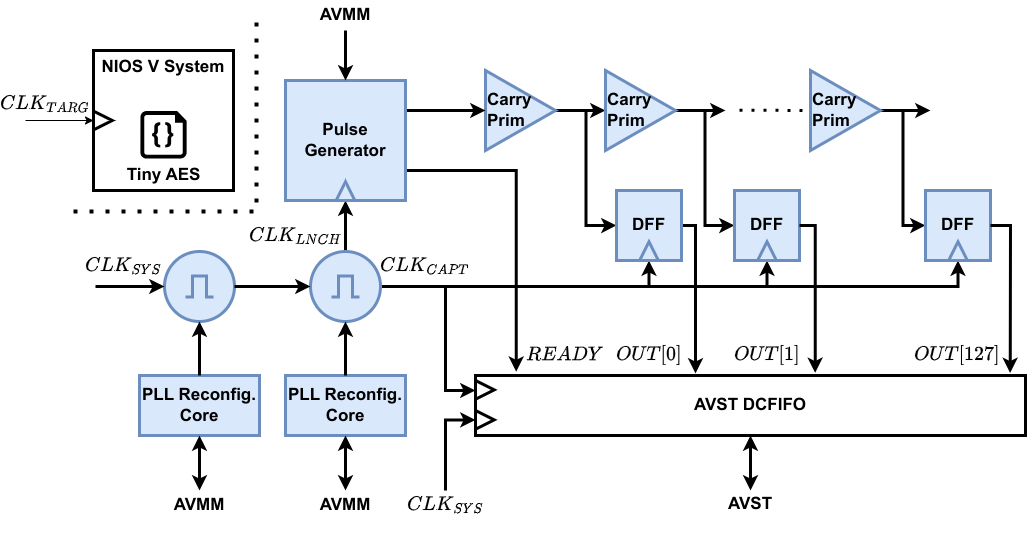
\includegraphics[width=\linewidth]{img/tunable_tdc_intel_sys.png}
  \caption{Intel tunable TDC voltage fluctuation sensor system architecture. The sensor core is highlighted in blue. Intel PLL reconfiguration cores replace the Xilinx MMCM enabling dynamic tuning of $\phi$ and $\theta$. All Avalon Memory-Mapped (AVMM) and Avalon Streaming (AVST) interfaces connect to the host CPU.  For characterization, a target NIOS-V (RISC-V) soft CPU core is implemented to execute a Tiny AES (AES-128) program. The target core is logically isolated and operates on a different clock domain than the voltage fluctuation sensor.}
\label{fig:tun_tdc_sys}
\end{figure} 

\section{Sensor overview}

The voltage fluctuation sensor demonstrated in
\cite{drewes2024pentimento} utilizes a TDC-based design. This feature
provides a mechanism for an adversary in a temporally multi-tenant FPGA
threat model to both measure fluctuations in propagation distance that
result from BTI-based stresses. Conceptually tuning the sensor can be
thought of as delaying the pulse through the tapped-delay-line of a TDC.
If the delay is too large the pulse will not travel through any of the
TDL delay elements, if it is too large the pulse will travel all the way
through the delay elements saturating the output. In both cases
measurements of propagation distance are clipped. To position the pulse
within the TDL, a tuning parameter $\theta$ is introduced as a phase
shift of the pulse into the TDC. For other attack classes such as the
measurement of voltage fluctuations for attacks in spatially
mutli-tenant threat models without losing the position of the tuned
input pulse, a secondary tuning parameter ($\phi$) is introduced which
corresponds to an equivalent phase shift of both the TDC input pulse and
the clock input to the TDC capture registers. Effectively tuning
$\theta$ corresponds to an adjustment of the observable TDL window,
while tuning $\phi$ corresponds to an adjustment of the position of the
window with respect to the target clock. The architecture of the tunable
dual-edge TDC implemented in this preliminary work is shown in Figure
\ref{fig:tun_tdc_sys}. The TDL is constructed from a chain of fast carry
elements where each carry primitive has a delay (shown below) of 6.4ps.
Two cascaded PLLs along with two Altera PLL Reconfiguration cores are
required to generate fine phase adjustment of both $\theta$ and $\phi$
parameters. Both PLLs are configured to 100MHz. A pulse generator
provides an input pulse at a rate of 25MHz. The capture registers will
capture both the rising and falling transition through the TDL making
this TDC implementation ``dual-edge". The dual-edge nature of this
sensor makes it more flexible as rising and falling transition
properties through the TDL may vary across technologies or board
vendors.

\section{Sensor design} Unfortunately, the phase step increment of Altera PLLs is 78ps,
introducing a fundamental design challenge. Current Altera FPGA product
families provide a minimum phase shift of $\frac{T_{VCOMAX}}{8}$. This
is significantly larger than the dynamic interpolated fine phase shift
minimum on Xilinx devices of $\frac{T_{VCOMAX}}{56}$. A lower minimum
phase shift results in a degradation of sensor resolution for both
tuning the observable window ($\theta$) and locating an area of maximum
information ($\phi$) for attacks on spatial co-tenants. To address this
limitation, a novel technique to construct a fine-grained phase sweep
from lower resolution phase shifts is proposed. This technique is
described in Algorithm \ref{alg:pll-intel}.

\setlength{\textfloatsep}{10pt} {
	\begin{algorithm}[t!]
		\footnotesize
		\caption{PLL configuration preprocessing for Altera FPGAs. Given a tuning parameter ($Tune \in \{\theta, \phi\}$), the TDC frequency ($F_{TDC}$), target frequency ($F_{TARGET}$), upstream PLL reference frequency ($F_{ref}$), and FPGA-dependent PLL counter, VCO, and PFD constraints ($Ms$, $Ns$, $Cs$, $F_{vco}^{min/max}$, $F_{pfd}^{min/max}$), compute PLL configurations spanning a range of phase-shift positions offset from either the launch clock ($\theta$) or the PLL initial phase ($\phi$).\label{alg:pll-intel}}
		\begin{algorithmic}[1]
			\Require $Tune$, $F_{TDC}$, $F_{TARGET}$, $F_{ref}$, $Ms$, $Ns$, $Cs$, $F_{vco}^{min/max}$, $F_{pfd}^{min/max}$
			\State $VCOs \gets Ms \times Ns$;\; $CFGs \gets \varnothing$; \Comment{cross-mult; valid cfgs.}
			\State $Max_{ph} \gets Tune\!=\!\theta \;?\; 1/F_{TDC} : 1/F_{TARGET}$;
			\ForAll{$(M,N) \in VCOs$}
			\State $F_{vco} \gets F_{ref}M/N$;\; $F_{pfd} \gets F_{ref}/N$;
			\If{$F_{vco} \notin [F_{vco}^{min}, F_{vco}^{max}] \,\lor\, F_{pfd} \notin [F_{pfd}^{min}, F_{pfd}^{max}]$}
			\State \textbf{continue}
			\EndIf
			\ForAll{$C \in Cs$ \textbf{s.t.} $F_{ref}M/(NC) = F_{TDC}$}
			\State $pb_d \gets 1/(8F_{vco})$;\; $n_{pb} \gets \lfloor Max_{ph}/pb_d \rfloor$; \Comment{min.\ phase bump (s); \# bumps}
			\ForAll{$pb \in \{1,\ldots,n_{pb}\}$}
			\State $delay \gets Tune\!=\!\theta \;?\; 1/F_{TDC} - pb\cdot pb_d : pb\cdot pb_d$;
			\State $CFGs.\texttt{append}(\{M, N, C, pb, delay\})$
			\EndFor
			\EndFor
			\EndFor
			\State $CFGs \gets \texttt{sort}(CFGs)$;\; $CFGs \gets \texttt{drop\_dup}(CFGs, delay)$; \Comment{sort by $M,N,C$, phase; dedup}
		\end{algorithmic}
	\end{algorithm}
}
\setlength{\textfloatsep}{10pt}

To improve the minimum phase shift for $\theta$ and $\phi$, every
possible phase shift increment is constructed by exhaustively iterating
through the space of all possible valid PLL configurations. A valid PLL
configuration must conform to the specifications provided by the part
manufacturer. For Cyclone V, the set of valid configurations must have
M, N, and C counters in the range of 1 to 512, a $F_{vco}$ in the range
of 600-1600MHz, and a $F_{pfd}$ in the range of 5-325MHz
\cite{intel_pll-spec}. From these valid configurations, all possible
phase shifts are determined either with respect to the launch clock or
the zero phase shifted position for $\theta$, and $\phi$, respectively.
This results in a much more fine grained (although variable) phase shift
resolution. Each PLL configuration will contribute varying power
consumption, phase noise and jitter due to the modification of the PLL
counters, VCO gain, loop filter and charge pump settings. Our results
indicate that the statistical methods used to tune $\theta$ and $\phi$
accommodate these perturbations, allowing us to adjust the position of
the observable window and identify an area of maximum information
despite the noise contributed by PLL reconfiguration. Note that there is
no additional target knowledge or a change of threat model from
\cite{drewes2024pentimento} to use Algorithm \ref{alg:pll-intel}.

\begin{figure}
\centering
  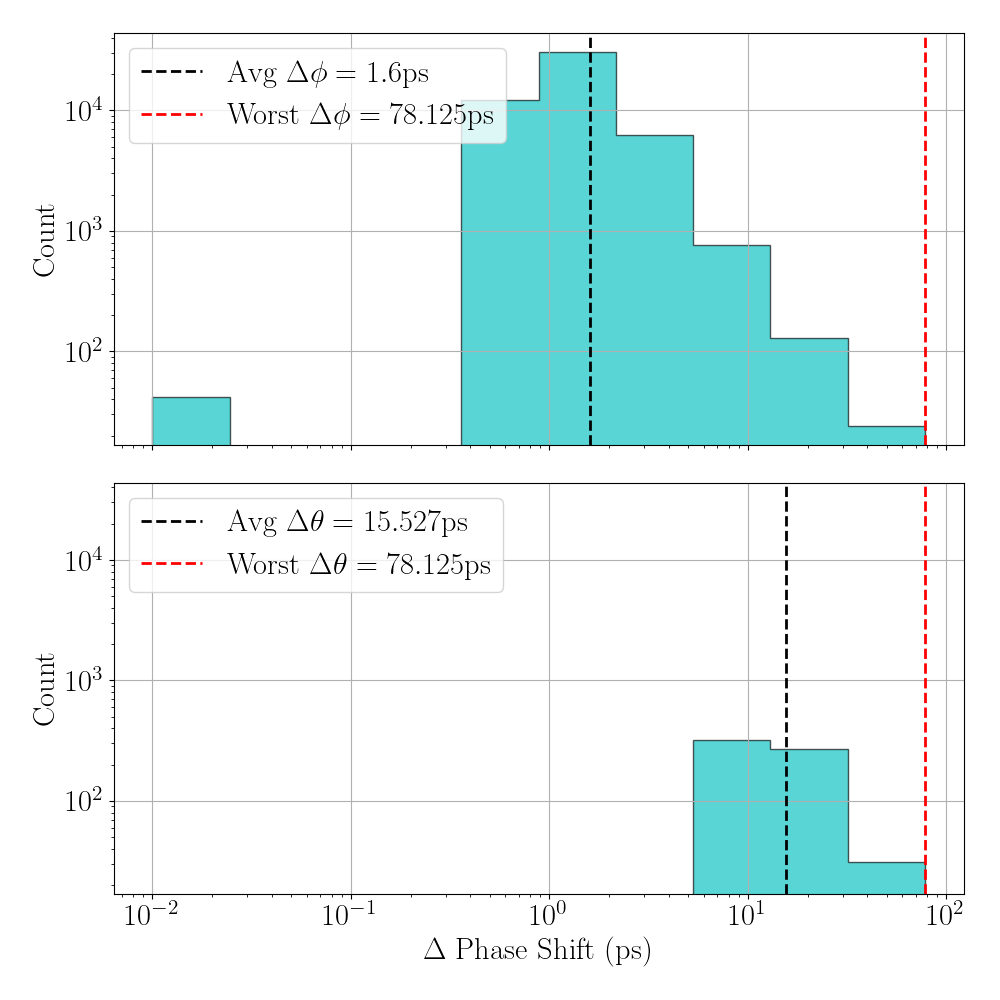
\includegraphics[width=0.70\linewidth]{img/ps_dist_intel.png}
  \caption{Distribution of phase-step granularity ($\Delta$ phase shift) for $\theta$ and $\phi$ with a fixed upstream clock generator output frequency of 10MHz and a fixed downstream clock generator output frequency of 100MHz. The worst-case phase shift is the minimum phase shift allowed by by the Intel PLL reconfiguration IP of 78.125ps. Utilizing the full space of valid counter configurations and phase shift increments for the PLL within the clock generator allows for a lower average phase shift amount. Phase shifting the upstream (downstream) PLL corresponds to an adjustment of $\phi$ ($\theta$). The range of $\phi$ phase shifts represented in the top histogram are generated from 0 to $4\pi$ and a 25MHz target clock (0-80000ps). The range of $\theta$ phase shifts represented in the bottom histogram is from 0 to $2\pi$ with the launch/capture capture clocks operating at 100MHz (0-10000ps).}
\label{fig:phase-shift-intel}
\end{figure} 

To maximize the sampling rate of the TDC, the downstream PLL should
operate at a maximum frequency. The upstream PLL can operate at many
frequencies without impact to the sampling rate. Fine adjustment is more
critical for $\phi$, as a user does not have control over the phase or
frequency of the target co-tenant logic. Figure
\ref{fig:phase-shift-intel} shows the distribution of minimum phase
increments for both $\theta$ and $\phi$ for a fixed upstream clock
generator frequency of 10MHz and fixed downstream frequency of 100MHz.
The minimum PLL phase shift of $\frac{T_{VCOMAX}}{8}=78.125ps$ becomes a
worst-case condition for both tuning parameters. However, on average,
our minimum phase shift improves for both $\theta$ and $\phi$ to 1.6ps
and 15.527ps, respectively. The upstream clock generator can operate at
a lower frequency, yielding more PLL arrangements for tuning $\phi$. The
downstream clock generator must provide a clock signal to the TDC logic
at 4 times the sensor sampling rate. This restriction presents a
trade-off between the sampling rate and the resolution of $\theta$. As
the PLL frequency scaling factor $\frac{F_{out}}{F_{ref}}$ is increased
given a fixed $F_{ref}$ there are fewer integer solutions to M, N, and O
in the equation $\frac{F_{out}}{F_{ref}}=\frac{M}{N*O}$. For example, in
our demonstrated PLL, half as many integer solutions exist to the
equation $\frac{100MHz}{10MHz} =\frac{M}{N*O}$ for M, N, and O bounded
to the range (1, 512) then there would be for $\frac{50MHz}{10MHz}
	=\frac{M}{N*O}$. Despite this trade-off, the proposed phase shifting
technique for $\theta$ still yields a significantly improved average
phase step resolution at a launch and capture clock rate of 100MHz
(25MHz TDC sampling rate).

\begin{figure}
\centering
\vspace{-12px}
\subfloat[\textit{First Index} metric]{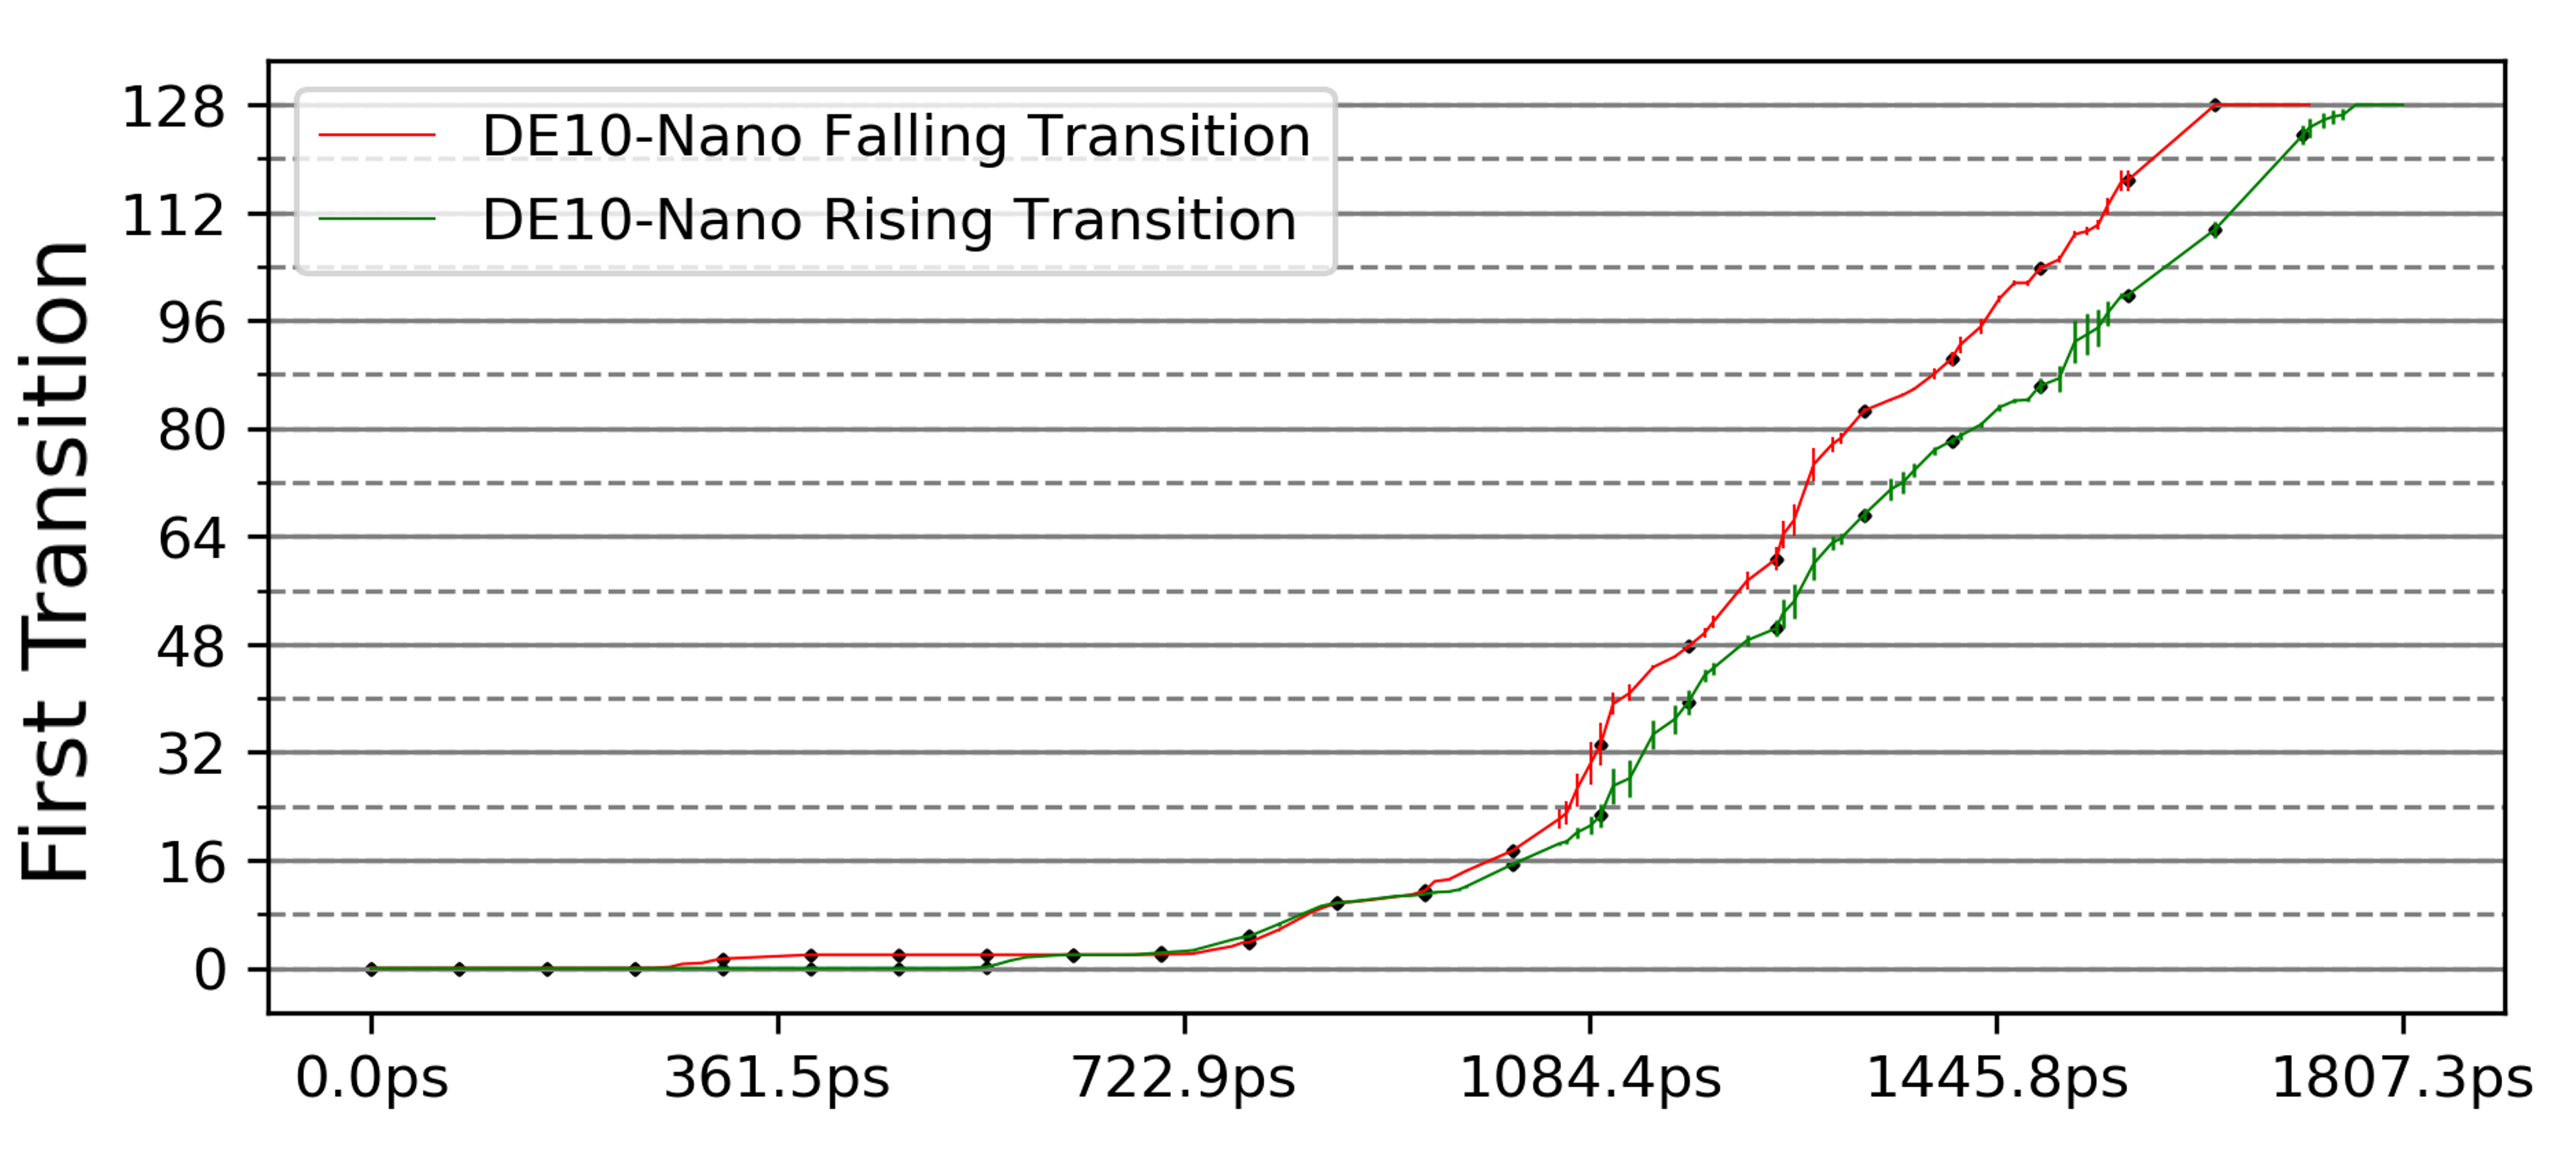
\includegraphics[width= 0.70\linewidth]{img/intel_first.png}\label{fig:prop-first-intel}}\\
\vspace{-12px}
\subfloat[\textit{Last Index} metric]{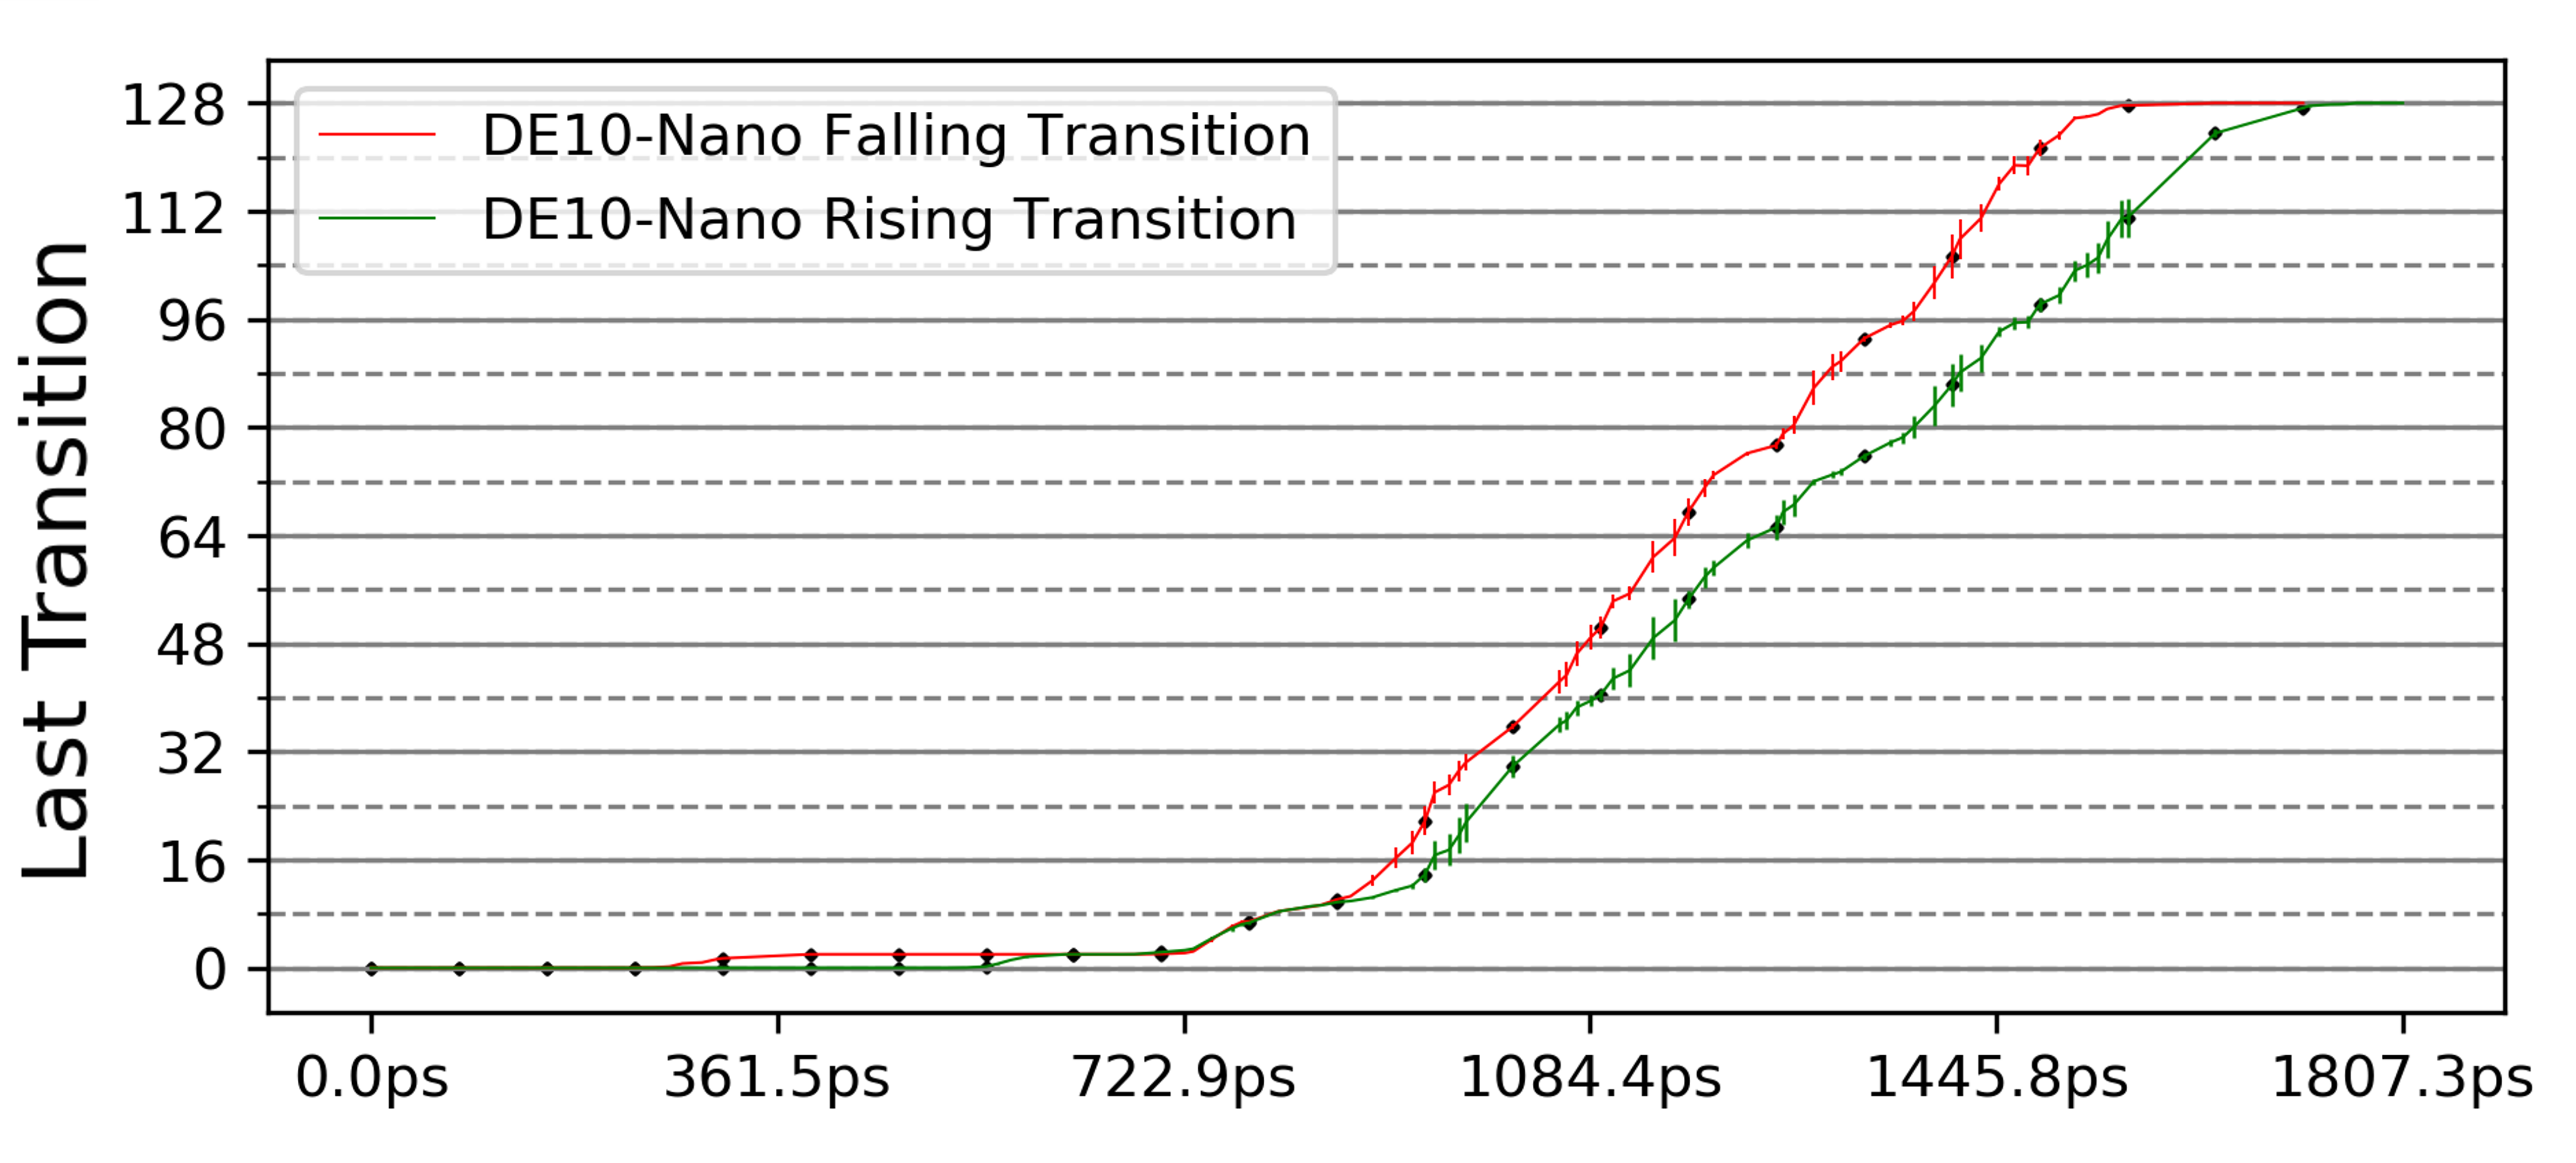
\includegraphics[width= 0.70\linewidth]{img/intel_last.png}\label{fig:prop-last-intel}}\\
\vspace{-12px}
\subfloat[\textit{Binary Hamming Distance} metric]{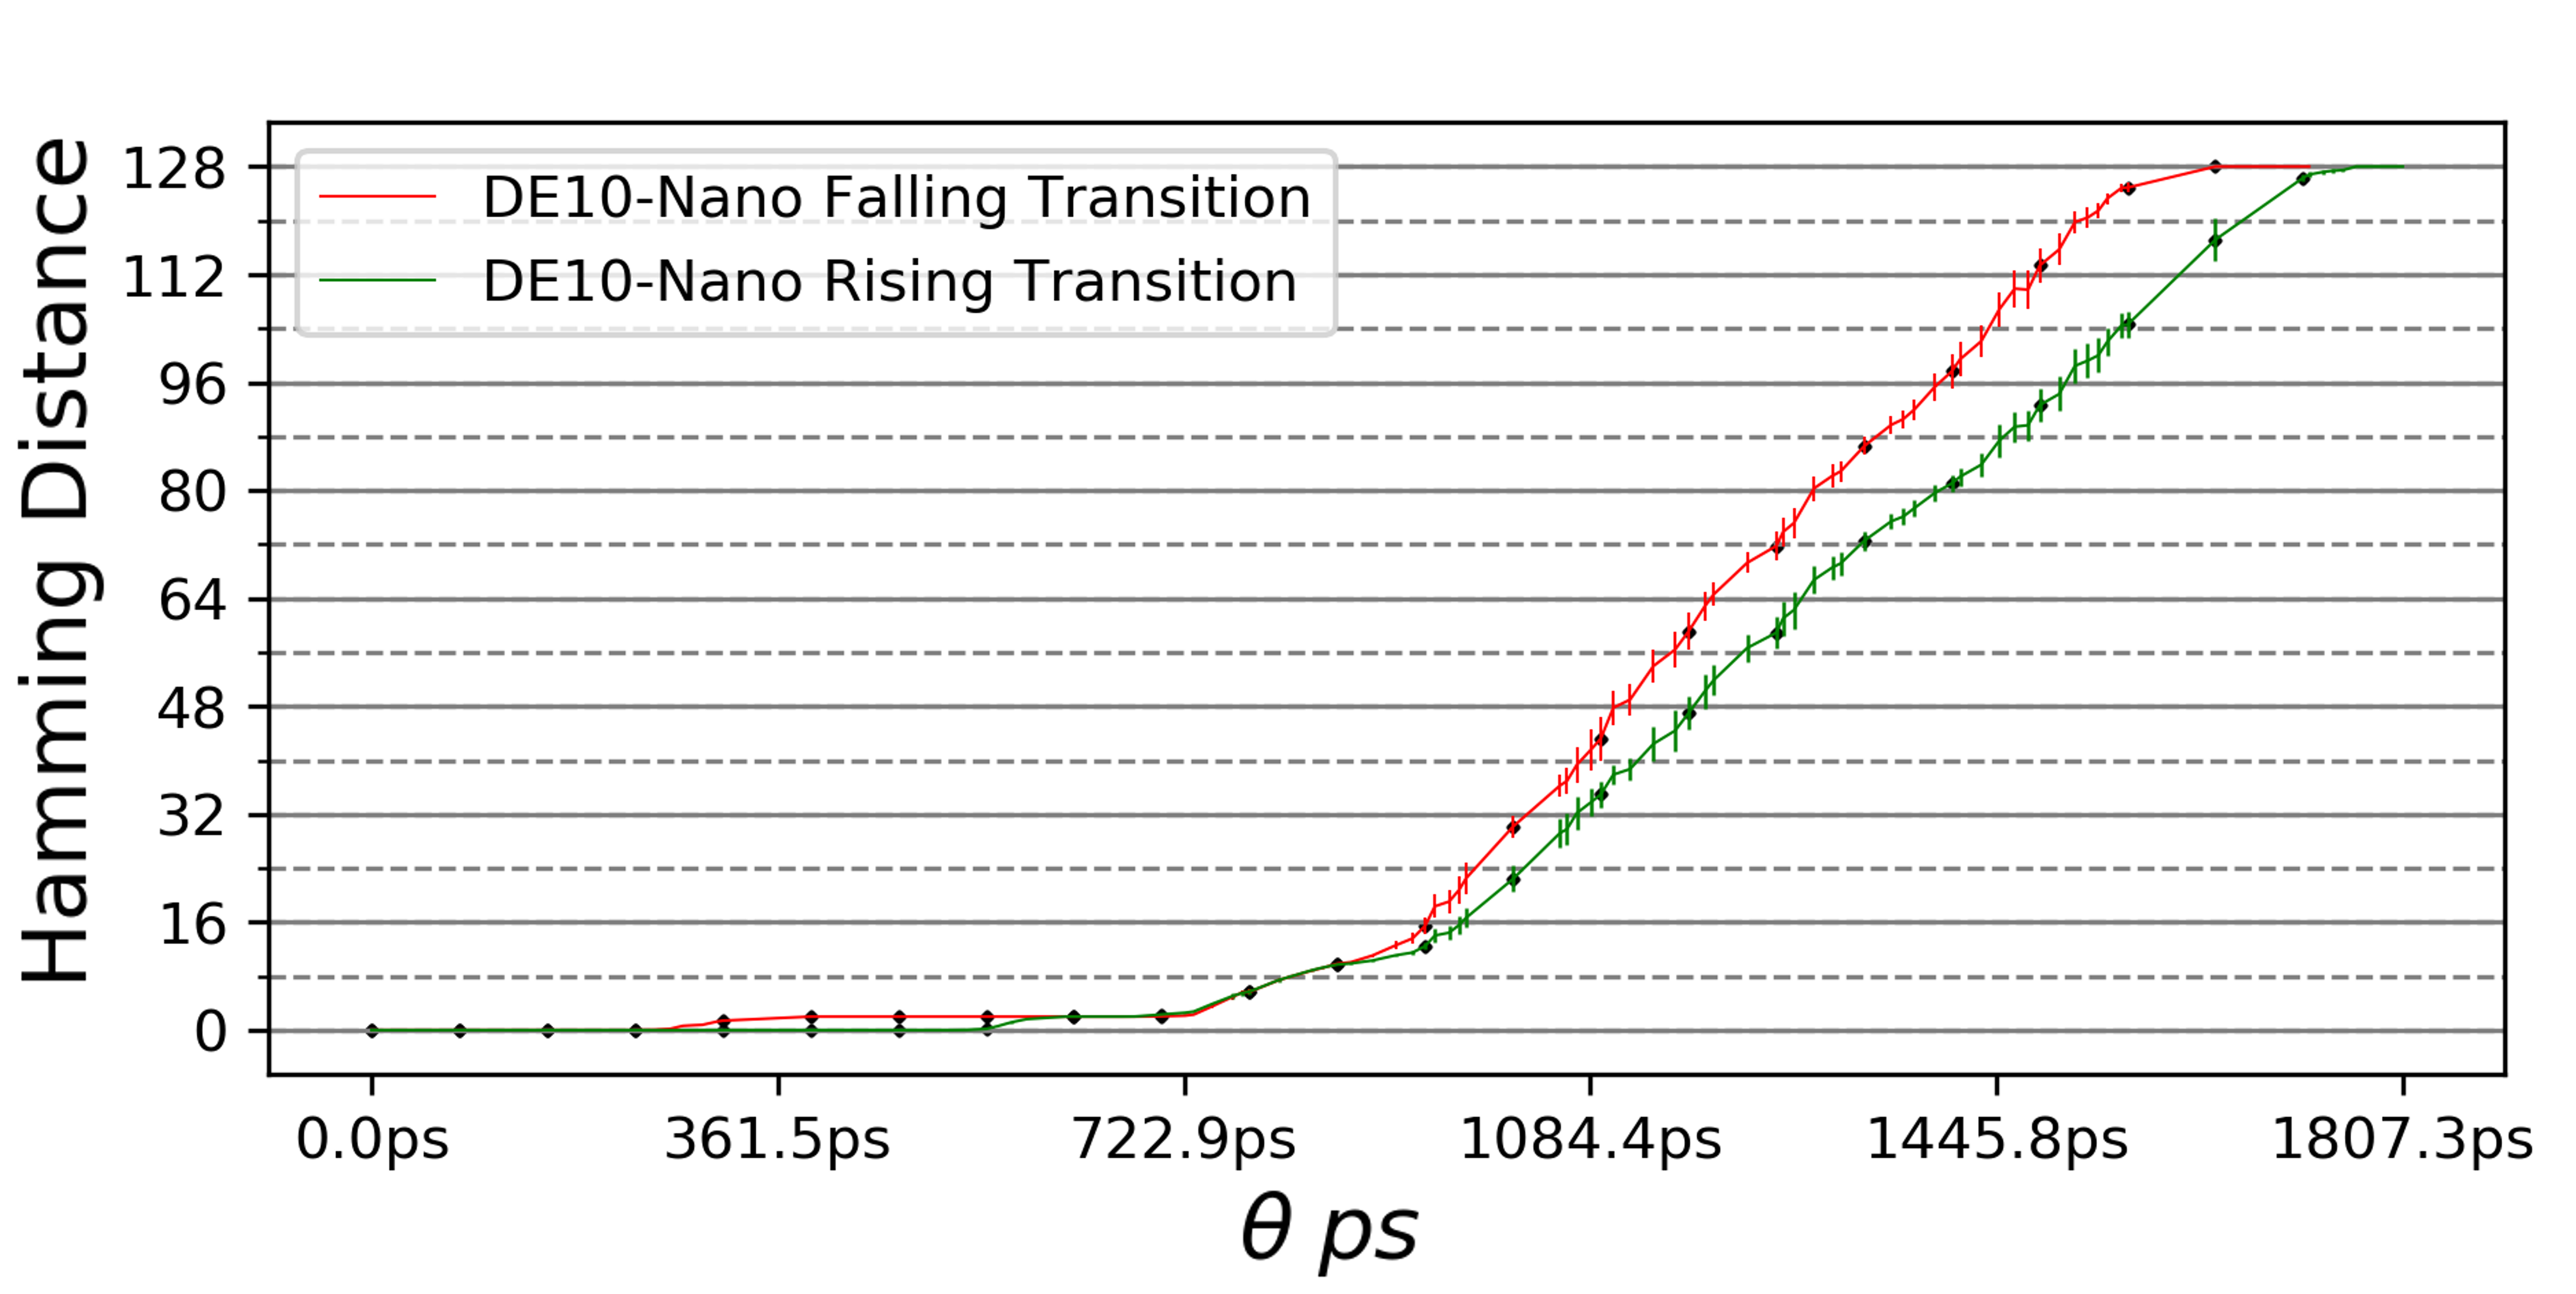
\includegraphics[width= 0.70\linewidth]{img/intel_ham.png}\label{fig:prop-pop-intel}}
\caption{Intel DE10-Nano propagation metrics for both polarities. Non-linearity in the propagation metric does not correspond directly to any known structure within the carry-chain as demonstrated on Xilinx. As demonstrated on Xilinx, hamming weight produces a significantly more linear propagation metric than the first and last transition metrics. The black diamonds represent the worst-case phase step increment and show the improvement in resolution achieved by our PLL configuration prepossessing algorithm.} %\cd{TODO - text bigger maybe. Combine x-axis to just bottom }} 
\label{fig:propagation-intel}
\end{figure}


Unique integer PLL configurations that produce identical output
frequencies do not produce equivalent phase noise, jitter, and power
consumption. However, with a sufficiently large sample sizes, these
noise sources do not impair the ability to tune $\phi$ and $\theta$.
Additionally, modifying integer PLL counters requires a reset to the
reconfigured PLL. This is not an issue for tuning $\theta$, as the phase
delay is measured between launch and capture clocks. However, $\phi$ is
measured from the zero phase shifted initial position of the PLL and
resetting the PLL can perturb $\phi$ tuning as resetting Altera PLLs
will erase all prior phase shift settings and results in a loss of PLL
lock. This limitation is described in greater detail below and a
solution is provided that resets the PLL only at the start of each
consecutive coarse-grained $\phi$ sweep.

\begin{figure}[t!]
\centering
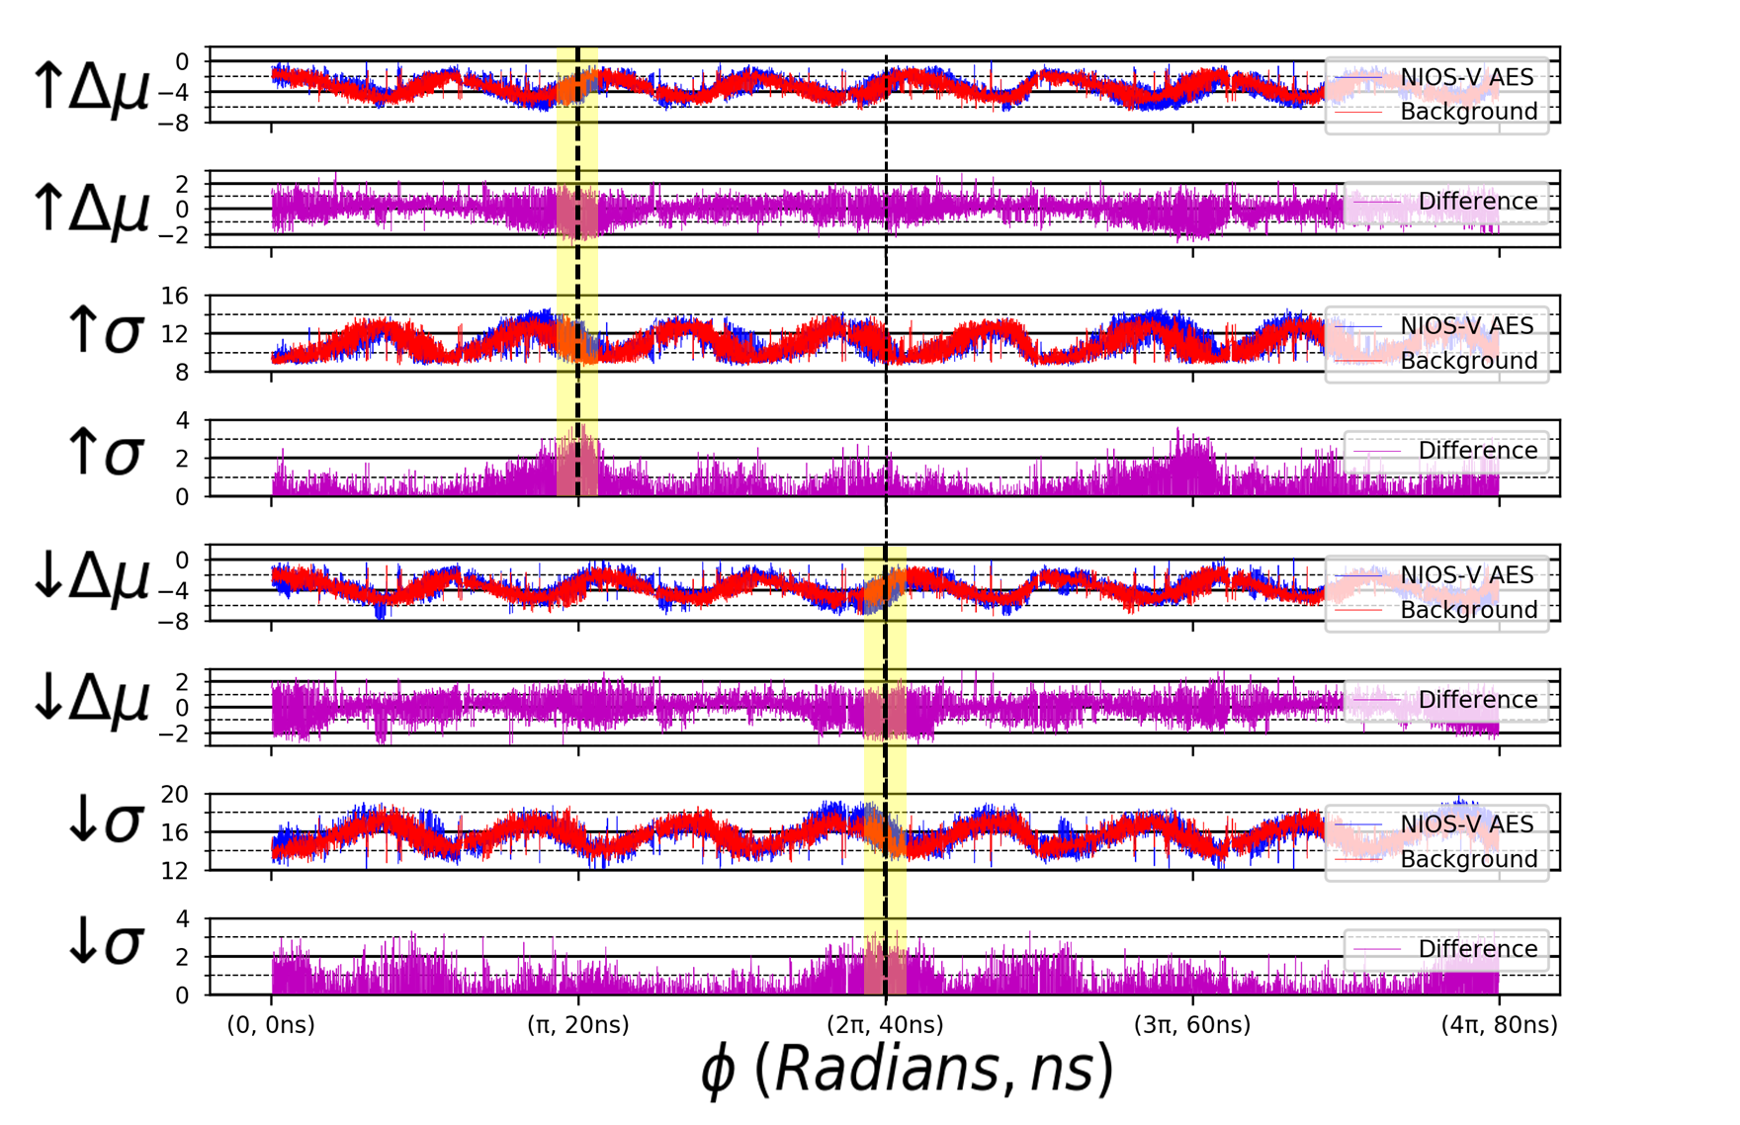
\includegraphics[width= 0.8\linewidth]{img/phi_sweep_niosv.png}
\caption{Measuring sensor output as $\phi$ is swept from 0 to 4$\pi$ on DE10-Nano NIOS-V/M design configured to run a AES-128 workload. The measured traces produce significantly more variance than the Xilinx systems, and we are able to isolate the power signature from the target NIOS-V core, and identify a region of maximum variance.\label{fig:phi-intel}} %\cd{TODO - text bigger maybe. Combine x-axis to just bottom }} 
\end{figure}

\section{Tuning $\theta$}
Figure \ref{fig:prop-pop-intel} demonstrates three different methods of
measuring propagation distance through the TDL. The propagation metrics
are used to encode TDL measurements. Due to clock skew, capture register
process variation and environmental effects, the value clocked into the
capture registers may be inconsistent with actual propagation distance.
The authors of \cite{prior} alleviate this effect by an investigation of
three propagation metrics. In the ``First" propagation metric,
propagation distance is defined as the first register to capture a
transition in the TDL. The ``Last" is defined as the last register to
capture the transition. And hamming weight is the total population count
with respect to the rising or falling transition. For example if a
rising pulse is registered as $0b1110110 \cdots 000$ and the pulse
enters the TDL MSB-first, then first metric would be 3, last would be 6,
and hamming weight would be 5. A falling transition with the captured
value $0b0001001 \cdots 111$ would have the same propagation distance
values. It is observed that the Hamming Weight metric has a smoothing
effect on each measurement, providing optimal linearity with respect to
the pulse input delay. It is noted in \cite{prior} that on Xilinx
architectures, the use of CARRY4 macros for TDL construction results in
plateaus appearing in the sensor outputs at the boundary of each CARRY4
macro. This is not observed to the same degree in the Altera
implementation. Additionally, steady variation is observed in all
regions of the TDL which is not the case for the Xilinx. Variation is
important as sensitivity to PDN fluctuations is a critical component to
remote RCS power side-channel attacks.

\section{Tuning $\phi$}

An Altera DE10-Nano system is programmed with a 128-bit instantiation of
the improved sensor, a hard processor system IP that interfaces the
Cylonce V FPGA to the co-packaged dual-core ARM A9 hard processor, and a
modular scatter-gather DMA engine to offload sensor readings to the
system memory. The launch and capture domains operate at 100MHz
($F_{sample}=25Mhz$). Instead of maximizing the internal $F_{vco}$ of
the PLLs within the clock generator modules, the phase step granularity
is improved using the PLL configuration prepossessing algorithm
described above. The output PLL configurations from the algorithm are
driven to the Altera PLL reconfiguration core for the upstream PLL as
consecutive coarse-grained phase sweeps. The measurements from each
coarse grained sweep are aggregated into a composite dataset that is
sorted with respect to the total phase offset of each measurement. This
procedure results in an effective phase-step granularity of 1.6ps as
shown in Figure \ref{fig:phase-shift-intel}.

To test the improved phase step resolution, the tunable TDC is
implemented alongside a NIOS-V/M soft CPU core on the DE10-Nano to
perform sensor characterization. Classification or other side-channel
attacks are not performed as identification of the active edge is
sufficient to verify. Instead, a more thorough description of the novel
phase-step techniques is provided and the runtime effects of this
technique on $\theta$ and $\phi$ tuning are described. To tune $\phi$,
an AES-128 workload is implemented on the NIOS-V/M core. When enabled,
the core will repeatedly perform decryption on a static plaintext.

Figure~\ref{fig:phi-intel} demonstrates the same experiment performed on
PYNQ-Z2 in \cite{prior} (with PicoV AES), instead on the DE10-Nano with
a NIOS-V/M design running a 25MHz clock frequency. In this experiment,
the improved phase-step resolution is utilized from the PLL
configuration prepossessing algorithm. Additionally, $\phi$ is swept
using subsets of coarse-grained sweeps described above. Much more
variance is observed in the trace when compared to the Xilinx systems
and the 25MHz NIOS-V/M target peak is clearly distinguishable. The
yellow highlighted region identifies where the channel contains maximum
information about the co-tenant NIOS-V/M core.

Sweeping $\phi$ using a set of PLL counter configurations requires
checks on the PLL lock status, and frequent resets of the clock
generators and sensor logic in the launch and capture clock domain.
These requirements are different from Xilinx where the only operations
performed on the clock generator PLLs are a minimum phase step
increment. In the Xilinx scheme, the cascaded PLLs of clock generator 1
and 2 can withstand small phase step increments on the upstream clock
generator without a loss of lock on the downstream clock generator. The
PLL configuration prepossessing algorithm improves the resolution of
$\theta$ and $\phi$ by using many PLL counter configurations with
varying $F_{vco}$ to produce a range of phase-step increments. While
this technique improves the average phase step, it requires
re-configuring the upstream PLL counters to make adjustments to $\phi$.
Altera PLL counter reconfiguration requires a reset to the PLL to
re-initiate the locking procedure. A reset to the clock generators
causes the pulse generator to no longer be synchronized with the initial
position of the $\phi$ sweep. This loss of synchronization distorts the
output. An alternative approach is to never reset during a sweep of
$\phi$ within the sweep measurement period (0 to $2\pi$ of the target
clock). To achieve this, we can describe our high resolution $\phi$
sweep as many composite coarse-grained $\phi$ sweeps.

Each coarse-grained sweep is identified by partitioning the set of PLL
configurations to matching counter values. These subsets can be
described as independent coarse-grained sweeps of $\phi$. The benefit to
performing many coarse-grained $\phi$ sweeps is that there is no
requirement for resetting the PLLs after initializing the counter values
of each coarse-grained sweep. Within each coarse-grained sweep only
phase bumps are performed on the upstream clock generator and if a loss
of lock occurs in the downstream generator we wait for it to relock
before sampling the sensor output. This allows the pulse generator in
the launch clock domain to remain stable during each coarse-grained
sweep. With this approach, it is possible to perform the composite
coarse-grained sweeps independently and overlay each coarse-grained
sweep result to produce the fine-grained $\phi$ result shown in Figure
\ref{fig:phi-intel}. Note that the peaks of the co-tenant clock are
clearly distinguishable, demonstrating that the Altera voltage
fluctuation sensor is able to achieve a fine-grained identification of
the target clock.

\section{Implications for FPGA Pentimenti}
\label{sec:fpga-pentimenti-implications}

The original FPGA Pentimenti demonstration~\cite{drewes2024pentimento}
was bounded by the phase-shift granularity of Xilinx MMCM primitives,
which expose dynamic phase steps at $T_{VCO}/56$. Intel Cyclone~V
exposes phase shifts only at $T_{VCO}/8$, an order of magnitude coarser,
and that coarseness was the practical reason no Intel demonstration of
the attack class had been attempted. The constrained PLL configuration
search introduced in this chapter shows that the coarse vendor primitive
is not a binding limit: by composing fine effective phase steps from
many valid integer PLL configurations, an average $\Delta \phi$ of 1.6ps
is achievable on Cyclone~V, finer than the Xilinx primitive and
sufficient for the picosecond-scale shifts characteristic of BTI-induced
pentimenti. The construction is not specific to Cyclone~V. Any FPGA
family whose default phase shift is set as $T_{VCO}/k$ for a small fixed
integer $k$, and whose PLL primitives expose dynamic counter
reconfiguration, allows the same approach. The number of valid integer
solutions to $F_{out}/F_{ref} = M/(N \cdot O)$ grows quickly as the
bounds on $(M, N, O)$ are widened.

This chapter demonstrates the sensor capability required for pentimenti
recovery on Intel platforms, not pentimenti recovery itself. Closing
that remaining gap requires characterization of the recoverable BTI
component on Cyclone~V's process node and verification that the
cumulative stress signatures targeted in \cite{drewes2024pentimento}
survive reconfiguration in the same manner. The mechanism underlying BTI
is shared across CMOS process nodes (Section~\ref{sec:bg-bti}), and the
measurement infrastructure to resolve its delay signature on Intel parts
has now been implemented.

